\chapter{Theory}

Before describing the work on friction estimates that has been done, it is important to have some knowledge within vehicle dynamics, including basic knowledge on how tires and also different differentials work. The following chapter tries to describe this so that the reader has the right basic knowledge needed.

\section{Vehicle dynamics}

When looking at vehicle dynamics, there are many variables that are interesting to know. Some of these include the vehicles yaw rate, and the lateral and longitudinal velocities and forces. The characteristics of a whole car is very complex and these parameters are therefore impossible to calculate exactly. There exists many different car models that try to describe the characteristics of a car as adequate as possible.If these calculations are supposed to be done on a cars computer, the model has to be simple enough to not reach the cars limited computing capacity.

\subsection{The bicycle model}

The bicycle model is a rather simple model that can be used to describe vehicle dynamics when turning, e.i. when we have a yaw rate and lateral forces that are affecting the vehicle. The models major simplifications consist of that the mass of the car is seen as one center of gravity point and that the two front wheels and the two rear wheels are combined into one wheel respectively as can be seen in Figure \ref{bicycle_model}. These simplifications lead to that there is no difference in normal forces on the two sides, e.i. there will be no roll  effect on the car when turning in a corner. There is also an assumption made that there will be no pitch effect on the car, which means that there is no suspension system that effecting the car. The model also assumes that there is no torque on the wheels, and therefore only lateral forces on the vehicle.

For most situations, these assumptions work fine, and the model gives a good idea on how different parameters are affected. Despite this, one has to bare in mind that these assumptions could result in rather large errors for certain driving situations.

\begin{figure}[h]
	\centering
	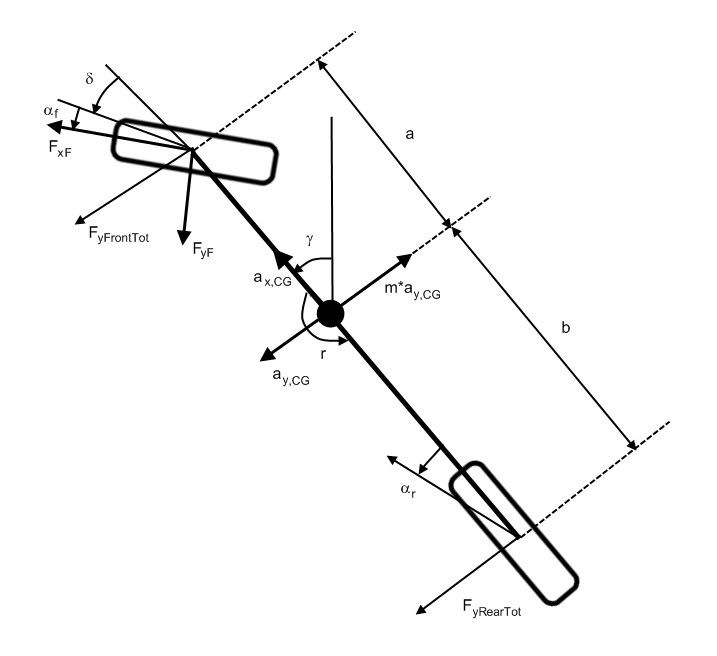
\includegraphics[width=0.8\textwidth]{Pictures/bicycle_model}
	\caption {Bicycle Model. \cite{fordonsdynamik99}}
	\label{bicycle_model}
\end{figure}

The total lateral force acting on the car will depend on the forces that the front and rear tires contribute with. By using Newtons second law of physics, $ F_{y} = m*a_{y} $, the lateral force on the car will be
\begin{equation} \label{eq:lateral_force}
	F_{y} = m*a_{y} = F_{yR} + cos(\delta)F_{yF} + sin(\delta)F_{xF} 
\end{equation}
where $ m $ denotes the vehicle mass, $ \delta $ is the front wheel steering angle and the acceleration in the center of gravity can be described as 
\begin{equation} \label{eq:lateral_acceleration}
	a_{y} = \dot v_{y} + \dfrac{F_{c}}{m}
\end{equation}
where $ \dot v_{y} $ is the actual change of velocity in lateral direction. The centrifugal force in the center of gravity, $ F_{c} $, depends on the yaw rate
\begin{equation} \label{eq:yaw_rate}
	\dot \Psi = \dfrac{v_{x}}{R}
\end{equation}
\begin{equation} \label{eq:centrifugal_force}
	F_{c} = \dfrac{m*v^2_{x}}{R} = mv_{x}*\dot \Psi
\end{equation}
Where $ R $ is the radius of the turning circle and $ v_{x} $ the velocity in x-direction in relation to the cars pointing direction. By combining Equations \ref{eq:lateral_acceleration} and \ref{eq:centrifugal_force}, the acceleration can described as
\begin{equation} \label{eq:lateral_acceleration_2}
	a_{y} = \dot v_{y} + v_{x}*\dot \Psi
\end{equation}

When combining Equations \ref{eq:lateral_acceleration_2} and \ref{eq:lateral_force} the different lateral force components can be described as
\begin{equation} \label{lateral_forces_2}
	F_{yR} + cos(\delta)F_{yF} + sin(\delta)F_{xF} = m*(\dot v_{y} + v_{x}\dot \Psi)
\end{equation}
If taken one step further, the lateral force components can describe the torque created around the z-axis in the center of gravity 
\begin{equation} \label{lateral_torque}
	M_{z} = I_{z}*\dot \Psi = a*(cos(\delta)F_{yF} + sin(\delta)F_{xF}) + b*F_{yR}
\end{equation}
where $ a $ and $ b $ are the lever lengths generated by the distances from the center of gravity to the front and rear axles respectively. 

When looking at the bicycle model,the assumption is that the longitudinal force is negligible. This means, as mentioned earlier, that the lateral force will almost only depend on the tire slip angle created by the front wheel steering angle and the angle to the direction the front wheel is heading towards. When assuming this model with only two wheels, the slip angles for the tires will be \cite{pacejka}

\begin{equation} \label{eq:wheel_slip_front}
	\alpha _{f} = -arctan(\dfrac{v_{y} + \dot \Psi *a}{v_{x}}) + \delta
\end{equation}

\begin{equation} \label{eq:wheel_slip_rear}
\alpha _{r} = -arctan(\dfrac{v_{y} - \dot \Psi *b}{v_{x}})
\end{equation}

\subsection{Normal forces}

The longitudinal and lateral forces that act on the tires are dependent on the normal forces. It is therefore interesting to know how much normal force that's acting on each tire.

\subsubsection{Lateral influence}

\begin{figure}[h]
	\centering
	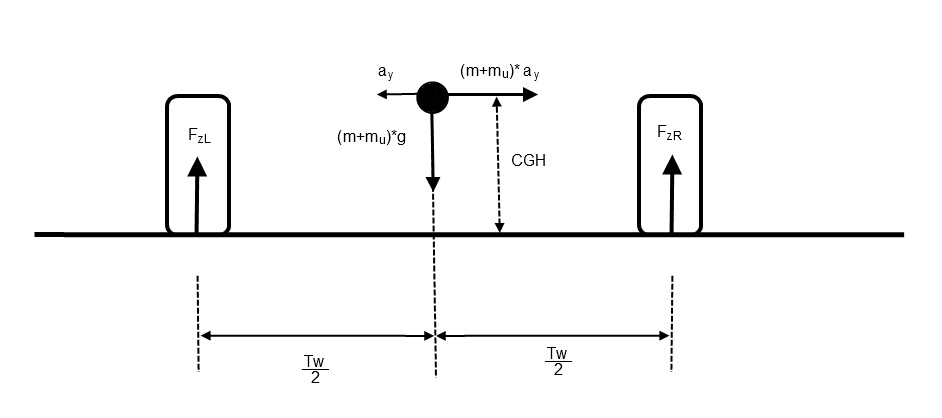
\includegraphics[width=0.8\textwidth]{Pictures/normal_force_lateral}
	\caption{Normal force on the car seen from the front.}
	\label{normal_force_lateral}
\end{figure}
Without any lateral acceleration, the right and left normal forces can be described as in Equation \ref{eq:normal}. 
\begin{equation} \label{eq:normal}
	F_{zL} + F_{zR} = mg
\end{equation}
With lateral acceleration, a torque will occur that changes the normal forces on the two sides. 
\begin{equation} \label{eq:normal_with_lat_acc}
	F_{zR}*T_{w} = mg*\frac{T_{w}}{2} + m*a_{y}*CGH
\end{equation}
The torque that affects the right side does in equation \ref{eq:normal_with_lat_acc} not take account for that the center of gravity height will change during driving.

When taking a corner, there will be load transfer from the inner to the outer wheel will depend on the centrifugal force and the load transfer coefficient $ \sigma_{i} $
\begin{equation}
	\Delta F_{zi} = \sigma_{i} ma_{y}
\end{equation}
\begin{equation}
	\sigma_{i} = \frac{1}{T_{w}}*( \frac{c_{\phi i}}{c_{\phi 1}+c_{\phi 2} - mgh'}h' + \frac{l-a_{i}}{l}h_{i}) 
\end{equation}
Where the \textit{i} denotes one of the axles (either front or rear), $ c $ the rolling stiffness, $ h $ the height from the ground to the axle, $ h' $ the distance from CoG to the roll axis, $ a_{1} = a $ and $ a_{2} = b $.

The final normal force on the front right wheel will be the normal force acting on the two front wheels divided by two, the unsprung mass of that one wheel, and the weight from the load transfer.
\begin{equation}
	F_{zFrontRight} = \frac{F_{zFront}}{2} + m_{UnsprungOneWheel}*g + \Delta F_{z}
\end{equation}
The problem with the calculations done above, is that the roll stiffness of both front and rear axle has to be known. The roll stiffness calculations are taken from \cite{pacejka}.



\subsubsection{Longitudinal influence}

\begin{figure}[h]
	\centering
	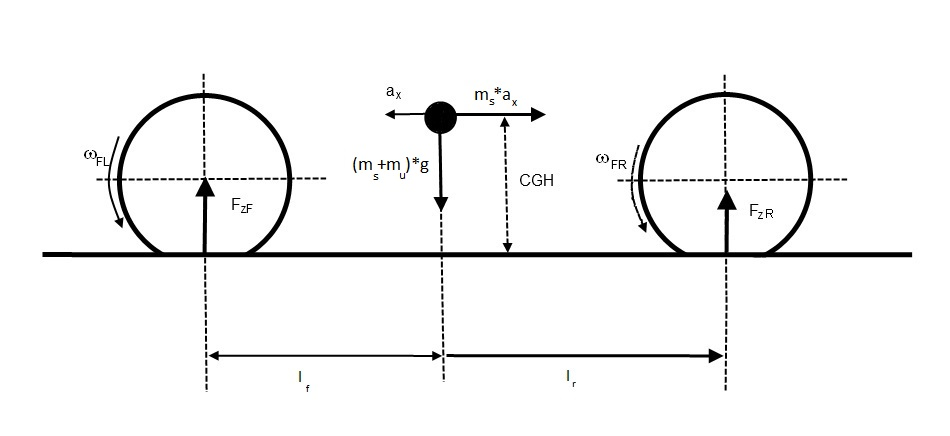
\includegraphics[width=0.8\textwidth]{Pictures/normal_force_longitudinal}
	\caption{Normal force on the car seen from the front.}
	\label{normal_force_longitudinal}
\end{figure}
\begin{equation} \label{eq:normal_2}
	F_{zF} + F_{zR} = mg
\end{equation}
\begin{equation} \label{eq:normal_with_long_acc}
	F_{zF}*(a+b) = mg*b - m*a_{x}*CGH
\end{equation}

For a car not in motion, the downward forces on the front and rear wheels will be equal to the gravitational force on the whole car. With longitudinal acceleration, the normal forces on the on the front respective the back will be changed, as can be seen in equation \ref{eq:normal_with_long_acc}. The normal force on the front will go down with positive acceleration. 

\section{Tire dynamics}
A gas inflated tire that is non loaded will have a radius called unloaded radius. When a tire is loaded, and therefore have a normal force acting on it from the road, it will deform against the road creating a contact area. The contact area is proportional to the load, more load gives larger contact area. The deformation of the tire will lead to a shorter distance between the center of the tire and the road, this is the loaded radius. 

A loaded tires contact area against the road can be divided into two, adhesion area and sliding area. The adhesion area is the part of the contact area that's said to adhere to the road, this means that this part haven't reached the friction limit yet, it can still handle more force without sliding. The sliding area is area that has reached the friction limit and thus has begun sliding. How this area is divided depends on a number of factors but it can basically be divided into two cases, longitudinal forces and lateral forces which will be explained further on.

\subsection{Longitudinal forces}
Rotating the tire will result in compression of the tire where the it hits the road and expansion where it leaves the road. The tire itself has a dampening effect meaning that all energy used to compress the tire won't be recovered when it expands again. This energy loss is called rolling resistance, $ R_{x} $. $ R_{x} $ is often modeled as being proportional to $ F_{z} $ with the proportionality constant $ f $ (Equation \ref{eq:rollingres}). A typical value of $ f $ is 0.015 for passenger cars \cite{rajamani}. The compression and expansion of the tire will also move the normal force acting on the tire in front of the center line (Figure \ref{rolling_resistance}) when the tire is rolling. The moved normal force will result in a third radius of the tire, the effective rolling radius. This is the radius related to the actual linear longitudinal velocity of the rolling tire, it's longer than the loaded radius but shorter than the unloaded radius.
\begin{equation}
R_{x} = fF_{z}
\label{eq:rollingres}
\end{equation}
\begin{figure}[h]
	\centering
	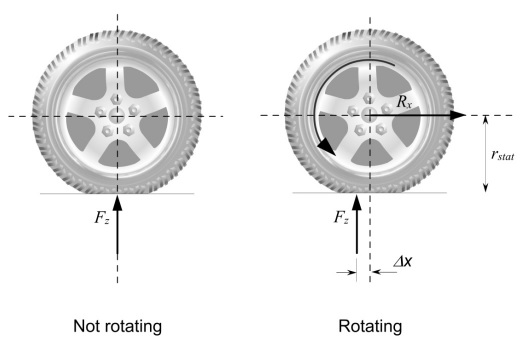
\includegraphics[width=0.8\textwidth]{Pictures/rolling_resistance}
	\caption{Normal force acting on the tire.}
	\label{rolling_resistance}
\end{figure}
When a longitudinal force is acting on the tire, traction or braking, the tire will have more compression/expansion and a slip will occur. The longitudinal slip, $ \kappa $ is defined as
\begin{equation}
\kappa = \dfrac{R_{e}\omega-V_{x}}{V_{x}}
\end{equation}
Where $V_{x}$ is the nominal velocity, $R_{e}$ the effective rolling radius, and $\omega$ the angular velocity of the wheel. This leads to the following slip with different angular velocities:
\begin{equation}
Braking: \omega = 0 \Rightarrow \kappa = -1
\end{equation}
\begin{equation}
Free rolling: \omega = \frac{V}{R_{e}} \Rightarrow \kappa = 0
\end{equation}
\begin{equation}
Spinning: \omega = 2\frac{V}{R_{e}} \Rightarrow \kappa = 1
\end{equation}
The longitudinal force that will be acquired depends on the normal force, $ F_{z} $ and the friction used, $ \mu(s) $.
\begin{equation}
F_{x} = F_{z}\mu(s)
\end{equation}
The used friction will increase with the slip ratio until the maximum friction is met. This is when full sliding occurs. 

\subsection{Lateral forces}

For a given slip angle one part of the contact area will adhere to the road and one part will slide against the road. The part that is sliding has reached the friction limit and the part that is adhering can still handle more force. As the slip angle increases a larger lateral force will occur forcing a bigger part of the contact area into the sliding region. At a certain slip angle the whole contact area will be in the sliding region. When this happens the lateral force for that tire has reached its maximum, turning more won't affect the vehicle anymore. This is well illustrated later on in \textit{Brush model (\ref{sec:brush})}.

Cornering stiffness
\begin{equation}
C_{y} = \frac{\delta F_{y}}{\delta}
\end{equation}
Where $\delta$ is the steering wheel angle.

Self aligning torque
\begin{equation}
M_{z} = F_{y}t_{p}
\end{equation}
Where $ F_{y} $  is the lateral force acting on the tire and $ t_{p} $ its distance to the center of the wheel. 

The lateral force acting on the wheel depends on its slip angle
\begin{equation}
F_{y}=C_{F}\alpha
\end{equation}
This can only be used in the linear part of the tire force/slip angle relationship. 

\section{Tire models}
There are several models to describe a tire mathematically. These models can be divided into four categories, empirical models, semi-empirical models, simple physical models and complex physical  models. 

Empirical models describe tire characteristics that are acquired from measurements of the tire. To fit the curve according to measured data the parameters are assessed with methods like regression. A well-known empirical model is the Magic Formula \cite{pacejka}. This model provides good fit for $F_{x}$, $F_{y}$ and $M_{z}$ curves and have coefficients that's easy to interpret.

Models using for example the similarity method are semi-empirical which means that some calculations are replaced by known or measured data. By distorting, rescaling and multiplying the result new relationships are acquired which can describe the tire in different situations. For example one can observe that that the pure slip curves shape doesn't change much \cite{pacejka} when the tire runs on different conditions. By shifting the nominal curve these conditions can be described.

The physical models are purely analytical and aims to describe the tire with the help of its physical characteristics. A simple physical model uses simple mechanical representation and can be calculated fairly easy by hand. This often results in pretty poor accuracy but sometimes that's enough. To get better accuracy a more complex model can be set up and simulated in a computer using aids like the finite element method. 

\begin{figure}[h]
	\centering
	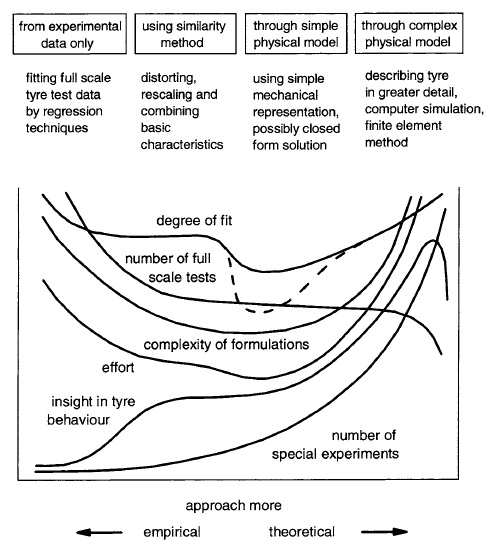
\includegraphics[width=0.8\textwidth]{Pictures/tire_modeling}
	\caption{Four categories of possible types of approach to develop a tire model. \cite{pacejka}}
	\label{tire_modeling}
\end{figure}

In Figure \ref{tire_modeling} some modeling characteristics and how they behave depending on category can be seen.

\subsection{Brush model}
\label{sec:brush}
The \textit{brush model} is a highly used \textit{simple physical model}. The idea is to model the tire surface as a row of elastic bristles that deflects in different directions depending on how the tire is loaded. This model is illustrated to the left in Figure \ref{brush1}.

\begin{figure}[h]
	\centering
	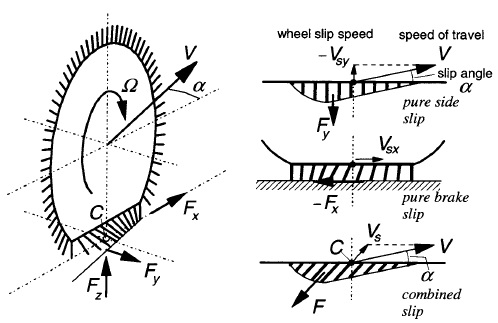
\includegraphics[width=0.8\textwidth]{Pictures/brush1}
	\caption{The brush tire model. \cite{pacejka}}
	\label{brush1}
\end{figure}

For pure side slip the bristles will deflect in the direction of the y-axis, this can be seen at the top right in Figure \ref{brush1}. In the same figure pure brake slip can be seen, that is when the bristles deflects in the direction of the x-axis. Finally at the bottom right of this figure combined slip is illustrated.

\begin{figure}[h]
	\centering
	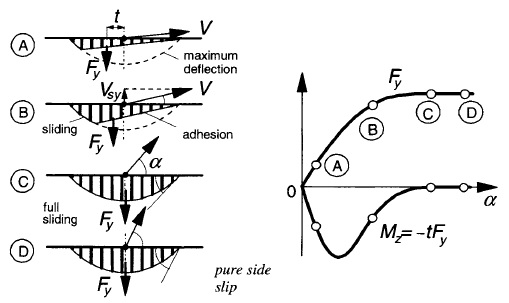
\includegraphics[width=0.8\textwidth]{Pictures/brush2}
	\caption{The brush tire model. \cite{pacejka}}
	\label{brush2}
\end{figure}

In Figure \ref{brush2} it can be seen how different slip angles affects the tire. Small slip angles gives a large adhesion area (flat part) and a small sliding area (curved part). As the slip angle increases a larger number of bristles reaches their maximum deflection, hence increasing the sliding area. At a certain slip angle all bristles have reached their maximum deflection and this results in full sliding. 

\subsection{Magic formula}

\section{Differentials}

\subsection{Open differential}

With an open differential, the torque will be evenly distributed on the two wheels, but the velocities can be different. This means that the inner wheel will have a lower velocity in a corner, due tu its smaller turning radius. When one wheel has significant lower resistant then the other, its velocity will become much higher due to the same amount of torque. Two possible scenarios for this is when you climb a hill with different friction on the two tires and when you take corner fast leading to the inner wheel lifting from the ground. Both of these scenarios will lead to very high speeds on the wheel on the low $ \mu $ surface respectively the inner lifting wheel. The torque that the non-spinning wheel can transfer to the ground will be the same amount that the spinning wheel can transfer, leading to significant lower traction than what actually is available on the wheels.

A solution in these different scenarios would be to lock the differential. This would lead to that the two wheels would have the exact same velocity, and therefore not the same torque in certain situations. 

Side-gear and crown wheel angular velocities:
\begin{equation}
	-1 = \frac{\omega_{1} - \omega_{r}}{\omega_{2} - \omega_{r}}
\end{equation}
\begin{equation}
	\omega_{r} = \frac{\omega_{1} + \omega_{2}}{2}
\end{equation}

\subsection{Limited slip differential}

The goal with a limited slip differential (LSD) is to not apply more torque to a wheel then it can transfer to the ground.

\subsection{FXD}

Does not create under steering like locking torque LSD's. 

Lightweight alternative  to improve traction performance. Very little extra fuel consumption. Pre-emptive lock torque for take off. Wheel slip control. Yaw damping. 

If ABS or ESP is active, the FXD function is shutout. 

"Side pull reduction"


\subsubsection{Control algorithm}

Signals available for the control algorithm through CAN:
\begin{itemize}
	\item 4x Wheel speeds
	\item Engine torque
	\item Engine speed
	\item Accelerator position
	\item Brake Pedal Active
	\item ABS active
	\item ESP torque request, opening request (slow/fast)
	\item Yaw rate
	\item Steering wheel angle
	\item Lateral acceleration
\end{itemize}

Other signals that are used are estimated:

Vehicle speed.
Tire size difference.
Tire stiffness???
Lateral acceleration???



\subsubsection{Applying pressure}

By applying higher current to the pump, it will spin faster and thus creating larger centrifugal forces. This force will block the oil from exiting the pump, leading to a higher pressure within the pump. This pressure is also applied to the clutch which will press the clutch discs together and locking the axles together.

\subsection{How differentials affect vehicle handling} 

\section{Tire/road friction models/methods}

There have been extensive research within this field for the last fifty years and this results in many different approaches to model tire/road friction. Some of the more relevant models/methods for this work will be presented here.

\subsection{Mue}

\begin{equation}
	\mu(F_{z})=\mu_{nominal}*(\mu_{max} + (-k)\frac{F_{z} - F_{z_{0}}}{F_{z_{0}}})
\end{equation}

\subsection{Slip-based friction model}
